\documentclass[10pt,aspectratio=169]{beamer}
\usepackage{tikz}
\usetheme{Boadilla}
\setbeamertemplate{navigation symbols}{}
\title{Iterative refinement: experiments and bounds}
\subtitle{Generated interaction study}
\author{Research group}
\date{}
\year=2026\month=11\day=5
\newcommand{\fuzzlayerA}[1]{\textrm{#1}}
\newcommand{\fuzzlayerB}[1]{\fuzzlayerA{#1}}
\newcommand{\fuzzterm}[1]{\fuzzlayerB{#1}}
\newcommand{\fuzzpair}[2]{\fuzzterm{#1}: #2}
\newcommand{\fuzzunit}{steps}
\let\fuzzoriginalunit\fuzzunit
\newcommand{\fuzzcoefficient}{4}
\newcommand{\fuzzscale}[2][\fuzzcoefficient]{#1\,#2}
\definecolor{fuzzpaint}{RGB}{255,0,255}
\definecolor{fuzzsecond}{RGB}{18,137,67}
\tikzset{fuzzvertex/.style={draw,rounded corners=1pt,fill=blue!10,inner sep=1pt,minimum width=.35cm,minimum height=.25cm}}
\begin{document}
\section{Iterative refinement}
\begin{frame}[t,shrink=5]{Iterative refinement}{Composed dependencies}
\fuzzpair{Experiment}{Timing: 12\fuzzunit; estimate $\fuzzscale{x}+\fuzzscale[2]{y}$.}\par
{\renewcommand{\fuzzunit}{samples}\let\fuzzterm\textbf\fuzzpair{LocalScope}{Timing: 7\fuzzunit.}\par}
\fuzzpair{RestoredScope}{Timing: 11\fuzzunit.}\par
\begin{block}{Iterative refinement}
\begin{itemize}
\item<1-> 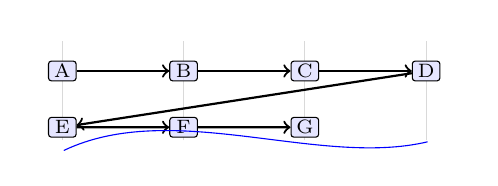
\begin{tikzpicture}[font=\scriptsize]
\begin{scope}[scale=1.1,rotate=0]
\clip (-.4,-1) rectangle (4.700,.5);
\foreach \x in {0,1,2,3} {\draw[gray!30] (\x*1.400,-.8)--(\x*1.400,.35);}
\node[fuzzvertex] (g3n0) at (0.000,0) {A};
\node[fuzzvertex] (g3n1) at (1.400,0) {B};
\node[fuzzvertex] (g3n2) at (2.800,0) {C};
\node[fuzzvertex] (g3n3) at (4.200,0) {D};
\node[fuzzvertex] (g3n4) at (0.000,-0.65) {E};
\node[fuzzvertex] (g3n5) at (1.400,-0.65) {F};
\node[fuzzvertex] (g3n6) at (2.800,-0.65) {G};
\begin{scope}[xshift=.5pt,yshift=-.5pt]
\draw<2->[->,thick] (g3n0) -- (g3n1);
\draw<2->[->,thick] (g3n1) -- (g3n2);
\draw<2->[->,thick] (g3n2) -- (g3n3);
\draw<2->[->,thick] (g3n3) -- (g3n4);
\draw<2->[->,thick] (g3n4) -- (g3n5);
\draw<2->[->,thick] (g3n5) -- (g3n6);
\draw[blue] (0,-.9) .. controls (1.260,-.3) and (2.940,-1.1) .. (4.200,-.8);
\end{scope}
\end{scope}
\end{tikzpicture}
\par
{\scriptsize\color{blue}\raggedright
\begin{enumerate}
\item<1-> \textbf{We compare the} proposed solution with a reference computed from the complete input. We compare the proposed solution with a reference computed from the complete input. The estimate is $\sum_{i=1}^{n}x_i$.
\item<2-> \textit{The final diagram} records the order in which information crosses the partition.  The estimate is $\sum_{i=1}^{n}x_i$.
\end{enumerate}\par}
\par
\begin{description}
\item[Stage 1] \textrm{Intermediate results carry} both a numerical estimate and an explicit dependency set. We compare the proposed solution with a reference computed from the complete input. The estimate is $\sum_{i=1}^{n}x_i$.
\item[Stage 2] \begin{tabular}{lrr}Method&Cost&Error\\\hline
Fresh0&21&28\\
Local1&15&19\\
Fresh2&1&15\\
Global3&11&13\\
\end{tabular}
\item[Stage 3] 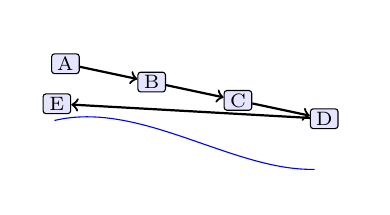
\begin{tikzpicture}[font=\scriptsize]
\begin{scope}[scale=0.8,rotate=-12]
\clip (-.4,-1) rectangle (4.700,.5);

\node[fuzzvertex] (g11n0) at (0.000,0) {A};
\node[fuzzvertex] (g11n1) at (1.400,0) {B};
\node[fuzzvertex] (g11n2) at (2.800,0) {C};
\node[fuzzvertex] (g11n3) at (4.200,0) {D};
\node[fuzzvertex] (g11n4) at (0.000,-0.65) {E};
\begin{scope}[xshift=.5pt,yshift=-.5pt]
\draw<1->[->,thick] (g11n0) -- (g11n1);
\draw<1->[->,thick] (g11n1) -- (g11n2);
\draw<1->[->,thick] (g11n2) -- (g11n3);
\draw<1->[->,thick] (g11n3) -- (g11n4);
\draw[blue] (0,-.9) .. controls (1.260,-.3) and (2.940,-1.1) .. (4.200,-.8);
\end{scope}
\end{scope}
\end{tikzpicture}
\end{description}
\item<2-> \begin{enumerate}
\item \begin{alertblock}{Constraint propagation}
\begin{itemize}
\item<1-> 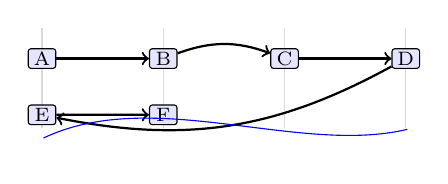
\begin{tikzpicture}[font=\scriptsize]
\begin{scope}[scale=1.1,rotate=0]

\foreach \x in {0,1,2,3} {\draw[gray!30] (\x*1.400,-.8)--(\x*1.400,.35);}
\node[fuzzvertex] (g15n0) at (0.000,0) {A};
\node[fuzzvertex] (g15n1) at (1.400,0) {B};
\node[fuzzvertex] (g15n2) at (2.800,0) {C};
\node[fuzzvertex] (g15n3) at (4.200,0) {D};
\node[fuzzvertex] (g15n4) at (0.000,-0.65) {E};
\node[fuzzvertex] (g15n5) at (1.400,-0.65) {F};
\begin{scope}[xshift=.5pt,yshift=-.5pt]
\draw<2->[->,thick] (g15n0) -- (g15n1);
\draw<2->[->,thick] (g15n1) to[bend left=20] (g15n2);
\draw<2->[->,thick] (g15n2) -- (g15n3);
\draw<2->[->,thick] (g15n3) to[bend left=20] (g15n4);
\draw<2->[->,thick] (g15n4) -- (g15n5);
\draw[blue] (0,-.9) .. controls (1.260,-.3) and (2.940,-1.1) .. (4.200,-.8);
\end{scope}
\end{scope}
\end{tikzpicture}
\item<2-> \begin{tabular}{lrr}Method&Cost&Error\\\hline
Local0&19&23\\
Cached1&15&7\\
\end{tabular}
\end{itemize}
\end{alertblock}
\item {\scriptsize\color{blue}\raggedleft
\begin{columns}[onlytextwidth,t]
\begin{column}{0.46\textwidth}
\textbf{A narrow column} can change line breaking even when the underlying expression is unchanged. The next pass must preserve the boundary conditions while revisiting dependent values. The estimate is $\frac{a+b}{1+c}$.
\end{column}
\begin{column}{0.50\textwidth}
\textit{A local update} can change the measurements used by several neighboring components.  The estimate is $\alpha+\beta$.
\end{column}
\end{columns}\par}
\item \begin{columns}[onlytextwidth,c]
\begin{column}{0.62\textwidth}
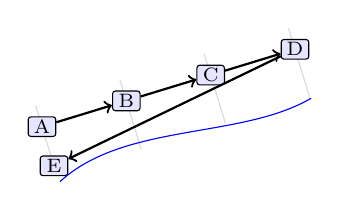
\begin{tikzpicture}[font=\scriptsize]
\begin{scope}[scale=0.8,rotate=17]

\foreach \x in {0,1,2,3} {\draw[gray!30] (\x*1.400,-.8)--(\x*1.400,.35);}
\node[fuzzvertex] (g22n0) at (0.000,0) {A};
\node[fuzzvertex] (g22n1) at (1.400,0) {B};
\node[fuzzvertex] (g22n2) at (2.800,0) {C};
\node[fuzzvertex] (g22n3) at (4.200,0) {D};
\node[fuzzvertex] (g22n4) at (0.000,-0.65) {E};
\begin{scope}[xshift=.5pt,yshift=-.5pt]
\draw<2->[->,thick] (g22n0) -- (g22n1);
\draw<2->[->,thick] (g22n1) -- (g22n2);
\draw<2->[->,thick] (g22n2) -- (g22n3);
\draw<2->[->,thick] (g22n3) -- (g22n4);
\draw[blue] (0,-.9) .. controls (1.260,-.3) and (2.940,-1.1) .. (4.200,-.8);
\end{scope}
\end{scope}
\end{tikzpicture}
\end{column}
\begin{column}{0.34\textwidth}
\begin{tabular}{lrr}Method&Cost&Error\\\hline
Fresh0&27&9\\
Cached1&0&13\\
Fresh2&24&8\\
Global3&23&29\\
\end{tabular}
\end{column}
\end{columns}
\end{enumerate}
\end{itemize}
\end{block}
\par 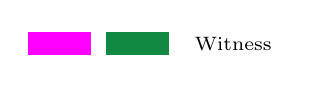
\begin{tikzpicture}[font=\scriptsize]
\fill<2-3>[fuzzpaint] (0,0) rectangle (.8,.3);
\fill<3->[fuzzsecond] (1,0) rectangle (1.8,.3);
\node[anchor=west] at (2,0.15) {Witness};
\end{tikzpicture}
\only<5>{}
\end{frame}
\renewcommand{\fuzzunit}{s}
\renewcommand{\fuzzcoefficient}{2}
\renewcommand{\fuzzterm}[1]{{\textbf{#1}}}
\section{Iterative refinement}
\begin{frame}[t]{Geometric uncertainty}
\fuzzpair{MacroStageB}{Timing: 12\fuzzunit, retained: 9\fuzzoriginalunit.}\par
{\renewcommand{\fuzzunit}{local}\fuzzpair{FrameLocal}{Timing: 5\fuzzunit.}\par}
\fuzzpair{FrameRestored}{Timing: 8\fuzzunit; estimate $\fuzzscale{x}$.}\par
\begin{columns}[T]\begin{column}{.46\textwidth}The next pass must preserve the boundary conditions while revisiting dependent values.\end{column}\begin{column}{.46\textwidth}\begin{itemize}\item Input state\item Updated state\end{itemize}\end{column}\end{columns}
\end{frame}
\end{document}
